%---------------
% Question 1
%---------------

\begin{question}{1}
\end{question}
\textbf{Example 2.2-1} describes a process in which a performance measure and
associated weights can be determined for controlling the attitude, $\theta(t)$,
of a manned spacecraft using a gas expulsion system, shown in Figure \ref{fig:spacecraft_acs}.
The objective of the control system is to maintain the attitude of the
spacecraft at $\theta(t) = 0$ with small accelerations.

\begin{figure}[H]
    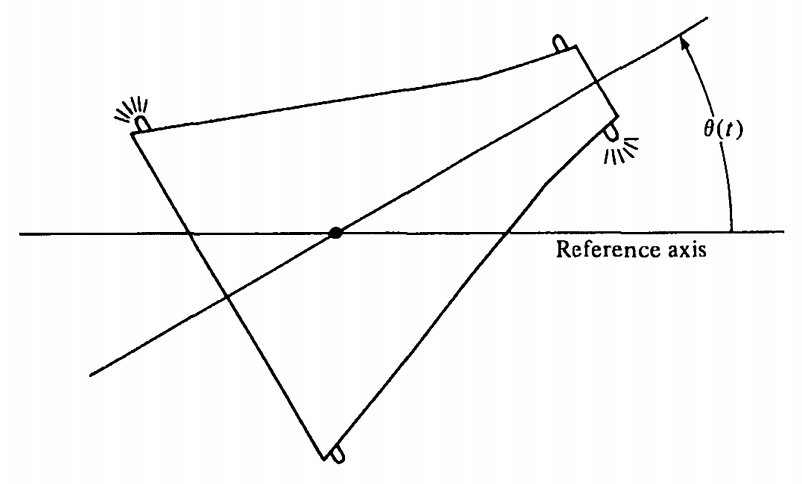
\includegraphics[scale=0.35]{spacecraft_acs}
    \centering
    \caption{Attitude control of a spacecraft \cite{kirkdover}}
    \label{fig:spacecraft_acs}
\end{figure}

The dynamics of the system are given by the differential equation given in
Equation \ref{eq:spacecraft_acs}.
\begin{equation}
    I \ddot{\theta}(t) = \lambda(t) \label{eq:spacecraft_acs}
\end{equation}

\noindent where $I$ is the angular moment of inertia and $\lambda(t)$ is the
torque produced by the gas jets. The state space equations are

\begin{align}
    \dot{x_1}(t) &= x_2 (t) \nonumber \\
    \dot{x_2}(t) &= u (t) \nonumber
\end{align}

\noindent where $u(t) = \dfrac{1}{I} \lambda(t)$ and the states, $x_1$ and
$x_2$, are angular position and velocity, respectively. The performance measure
is given in Equation \ref{eq:spacecraft_pf1} below

\begin{equation}
    J = \int_{0}^{\infty} [q_{11} x_1^2(t) + q_{22} x_2^2(t) + R u^2 (t)] \, dt
    \label{eq:spacecraft_pf1}
\end{equation}

\noindent where $q_{11}$, $q_{22}$, and $R$ are the weights.

To find specific values of the weights, we must take into account the desired
qualities of the controller. In this problem it desired to maintain a specific
attitude and to do so using small accelerations. This means that we are
concerned with $x_1(t)$ and with $u(t)$. Therefore, our weighting matrix, $Q$,
can be defined as

\begin{equation} \label{eq:sc_q}
    Q \, = \,
    \begin{bmatrix}
        q_{11} & 0 \\
        0      & 0
    \end{bmatrix}
\end{equation}

Notice in Equation \ref{eq:sc_q} that all entries \textit{except} the $q_{11}$
entry are $0$. This is because the only state that is to be given any
preference is the $x_1$ state, which corresponds to the $q_{11}$ entry. We're
also concerned about the acceleration which is the control action, $u(t)$, in
this case. Because $u(t)$ is not a vector, or $R \, \in \, \mathbb{R}$, and all
of the entries of $Q$ are $0$ except for $q_{11}$, Equation
\ref{eq:spacecraft_pf1} can be rewritten as

\begin{equation}
    J = \int_{0}^{\infty} [q_{11} x_1^2(t) + R u^2 (t)] \, dt
    \label{eq:spacecraft_pf2}
\end{equation}

Now, we can see how choosing particular values for $q_{11}$ and $R$ affect
system performance. Let's focus only on differing values of $R$. Throughout,
we'll use the following conditions for $Q$ and $X_0$

\begin{equation} \label{eq:sc_params}
    Q \, = \,
    \begin{bmatrix}
        4 & 0 \\
        0 & 0
    \end{bmatrix}
    , \quad
    X_0 \, = \,
    \begin{bmatrix}
        10 \\
        0
    \end{bmatrix} \nonumber
\end{equation}

Figure \ref{fig:sc_low} shows the response of the system with $R = 0.1$.
Because $R$ is a small value, its resonse is given less preference which
results in a large acceleration (control action). The large acceleration in
turn results in large overshoot along with the spacecraft quickly settling on
its desired attitude of $\ang{0}$. A fast response is not what we want as it
could injure or make the astronauts that are inside the spacecraft ill.

\begin{figure}[H]
    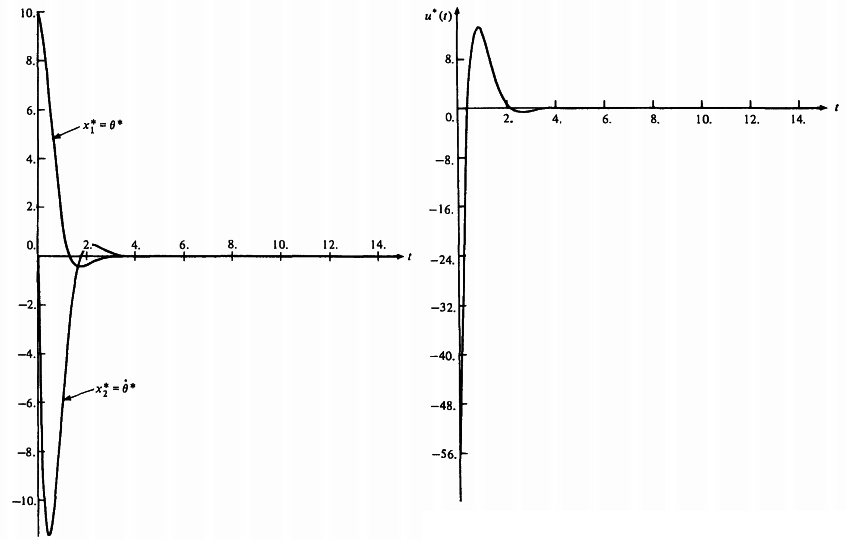
\includegraphics[scale=0.4]{sc_low}
    \centering
    \caption{Response of system with $R = 0.1$ \cite{kirkdover}}
    \label{fig:sc_low}
\end{figure}

Figure \ref{fig:sc_med} shows the response of the system with $R = 1$.
Because $R$ is a larger value than in the previous configuration, its resonse
is given more preference which results in a smaller acceleration. This smaller
acceleration in turn results in a smaller overshoot and the spacecraft settling
on its desired attitude of $\ang{0}$ slower than before (longer settling time).

\begin{figure}[H]
    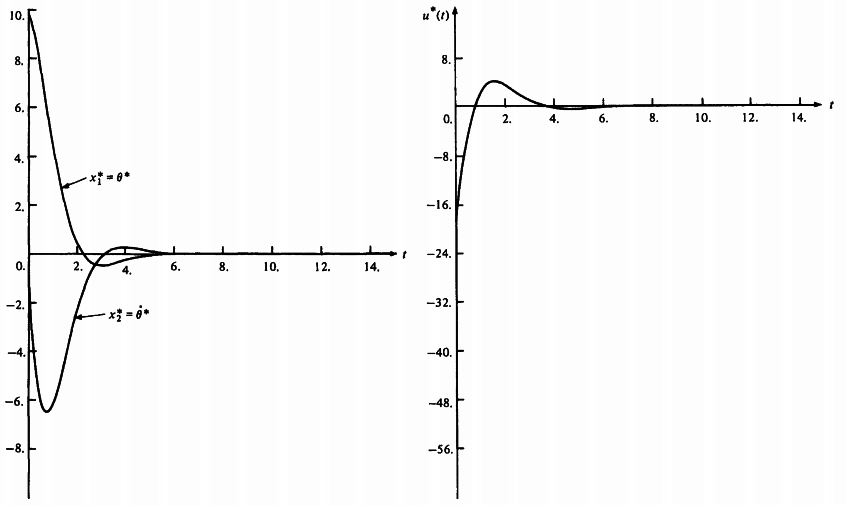
\includegraphics[scale=0.4]{sc_med}
    \centering
    \caption{Response of system with $R = 1$ \cite{kirkdover}}
    \label{fig:sc_med}
\end{figure}

Figure \ref{fig:sc_high} shows the response of the system with $R = 10$.
Because $R$ is a much larger value than the first configuration (100 times as
large), its control action was given much more preference and the control
history and state trajectories that are generated are much closer to the
requirements. The overshoot is considerably smaller than in the first
configuration ($R = 0.1$) and its settling time is also much longer.

\begin{figure}[H]
    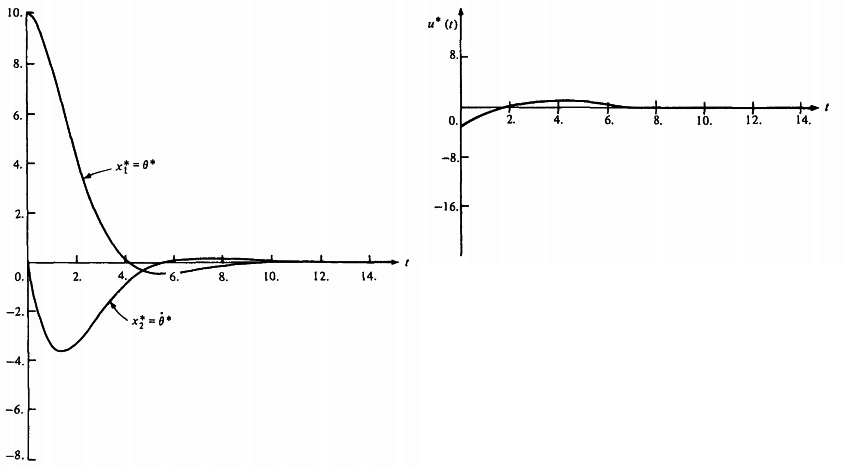
\includegraphics[scale=0.4]{sc_high}
    \centering
    \caption{Response of system with $R = 10$ \cite{kirkdover}}
    \label{fig:sc_high}
\end{figure}

What \textbf{Example 2.2-1} shows is that giving larger weights to a parameter
in the performance measure causes that parameter to be given more
consideration by the controller. This allows control engineers to tune their
controllers to give the desired performance.
